\chapter{常见误区}
\label{chap:21}

\begin{chapteropening}
“单光子”“纠缠”“超分辨”“非 Poisson”“新物理”这些词很容易把问题说得过大。数据本身要更具体：事件表怎样变成联合概率，相关峰怎样标定，假警报怎样计算，模型参数在哪些条件下还能估计。本章按同一诊断顺序展开：先指出容易误读的说法，再写出真正的观测量，最后给出校准项、系统误差或 trial factor。量子光学的基本判据、强度干涉的天文实现、SPADE 的信息极限、天体 maser/laser 和天文统计检验分别见 \citet{1963PhRv..130.2529G,1963PhRvL..10..277S,1965RvMP...37..231M,1977PhRvL..39..691K,1985stop.book.....G,1995ocqo.book.....M,1956Natur.178.1046H,1957RSPSA.242..300B,1974iiia.book.....H,2020NatAs...4.1164A,2016PhRvX...6c1033T,1992ARA&A..30...75E,1979ApJ...228..939C,2013ApJ...764..167S}。
\end{chapteropening}

\section{看到光子为什么不等于量子天文学}

单光子探测器只是数据入口。若分析只把第 \ref{chap:01} 章式 \eqref{eq:event-row} 的事件表求和成平均计数率 \(R=N_\gamma/T\)，得到的仍然是普通光变曲线。量子天文学中新增的信息来自事件之间的联合分布，最简单的独立情形、二阶相关和 pair count 已在第 \ref{chap:02} 章式 \eqref{eq:ch02-independent} 和 \eqref{eq:ch02-g2-count} 中建立。判断一个分析是否用到了事件表，要看标签有没有进入模型：\(t\) 是到达时间，单位 s 或 ns；\(d\) 是探测器/望远镜编号；\(\nu\) 是频率通道，单位 Hz 或通道号；\(p\) 是偏振标签。若这些标签在分析时全部被丢掉，仅凭探测器能数单光子还不足以声称测到了新的量子观测量。

一个常见错误是把“低光子数”直接等同于“量子”。X 射线和伽马射线天文学长期使用 Poisson 计数和 Cash 似然，但许多问题仍只是平均强度或能谱估计 \citep{1979ApJ...228..939C,1986ApJ...303..336G}。反过来，射电和毫米波常处在高占有数、近经典波动极限，却仍能讨论相干函数、相位、偏振和量子噪声。判据在于模型是否需要多光子联合概率或光场模式来表达。

事件表也不会自动产生新物理。Poisson 计数模型已经在第 \ref{chap:01} 章式 \eqref{eq:poisson} 给出，分箱版本见第 \ref{chap:07} 章式 \eqref{eq:ch07-binned-poisson}。\(\mu_k=R_k\Delta t_k\) 是第 \(k\) 个 bin 的期望计数，没有单位。若源本来在变，\(\mu_k\) 也随时间变；若有效曝光 \(E_k\) 因云、死时间或选择函数改变，\(\mu_k\) 应写成 \(R_kE_k\Delta t_k\)。把所有 \(N_k\) 和一个常数 \(\mu\) 比较，然后宣布“非 Poisson”，通常只是把普通光变、坏天气或曝光变化误当作统计异常。Bayesian Blocks、周期搜索和似然比检验都能处理这类问题，但每种方法有自己的适用条件和试验次数 \citep{1982ApJ...263..835S,1992ApJ...398..146G,2002ApJ...571..545P,2013ApJ...764..167S}。

\section{\texorpdfstring{为什么 \(g^{(2)}=1\)}{为什么 g2=1} 不是充分判据}

\(g^{(2)}(0)=1\) 常被误说成“光一定是经典激光”，或者反过来被误说成“没有量子性”。相干态给 Poisson 光子数分布和 \(g^{(2)}(0)=1\)，但 \(g^{(2)}(0)=1\) 不是相干态的唯一指纹。多模热光在模式数 \(M\) 很大时也会接近 1；有限时间响应还会继续稀释聚束峰。对比度稀释的基本形式见第 \ref{chap:04} 章式 \eqref{eq:ch04-contrast-dilution}。\(\tau_c\) 是相干时间，单位 s；\(\Delta t_{\rm eff}\) 是探测器响应或相关 bin 的有效宽度，单位 s；有效模式数 \(M_{\rm eff}\) 包括空间、频率、偏振和时间模式。可见光 \(10\,{\rm nm}\) 带宽在 \(500\,{\rm nm}\) 附近给 \(\tau_c\sim10^{-14}\,{\rm s}\)，而电子学 bin 常是 \(10^{-9}\)--\(10^{-8}\,{\rm s}\)。即使 \(M_{\rm eff}=1\)，对比度也只有 \(10^{-6}\)--\(10^{-5}\)。Guerin 的星光聚束实验、AQuEye/IquEye 方案和 VERITAS/MAGIC 强度干涉都把这个稀释作为核心量处理 \citep{2017MNRAS.472.4126G,2016SPIE.9907E..0NZ,2020NatAs...4.1164A,2021MNRAS.506.1585Z,2024MNRAS.529.4387A,2024ApJ...966...28A}。

\begin{figure}[tbp]
\centering
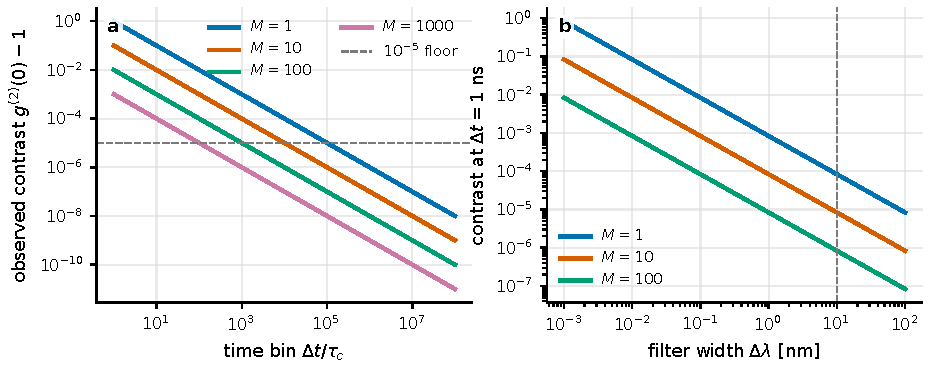
\includegraphics[width=0.96\linewidth]{figures/generated/chapter_21/ch21_g2_scaling_mistake.pdf}
\caption{时间 bin、光谱带宽和模式数对 \(g^{(2)}\) 对比度的稀释。左图显示 \(\Delta t/\tau_c\) 和 \(M_{\rm eff}\) 如何把单模热光的聚束峰压低；虚线表示 \(10^{-5}\) 级系统误差地板。右图把滤光片带宽换成相干时间，在 \(1\,{\rm ns}\) 采样下，宽带可见光的热光峰很容易低于可校准范围。}
\label{fig:ch21-g2-scaling}
\end{figure}

反聚束比 \(g^{(2)}=1\) 更强，因为 \(g^{(2)}(0)<1\) 不能由经典随机强度给出。Kimble、Dagenais 和 Mandel 的共振荧光实验是这个判据的经典例子 \citep{1977PhRvL..39..691K}。天体光源中要看到反聚束极难：光源通常由大量独立发射体、传播路径和探测器响应混合，任何单个量子发射体的亚 Poisson 特征都会被空间、频率和时间平均稀释。因此天文报告若写“\(g^{(2)}\simeq1\)，所以是激光”或“\(g^{(2)}\simeq1\)，所以没有量子信息”，都没有足够依据。

\section{强度干涉为什么仍然需要校准}

强度干涉对大气 piston 相位不敏感，但校准仍然决定相关幅度。透明度、闪烁、镜面反射率、滤光片形状、光电倍增管增益、SPAD 死时间、电子串扰和背景光都会进入相关幅度。一个实用的数据模型可以写成
\begin{equation}
  \hat c_b(\tau)=
  \beta_b\,|V_b|^2\,h_b(\tau)
  +c_{{\rm inst},b}(\tau)
  +c_{{\rm sel},b}(\tau)
  +\epsilon_b(\tau).
  \label{eq:ch21-calibration-model}
\end{equation}
\begin{formulaexplain}[公式 (21.1) 解读]
\(\hat c_b\) 是实测相关超额。第一项是天体信号，后面依次是仪器项、选择项和随机误差；强度干涉不怕大气相位，却仍怕这些幅度校准项。
\end{formulaexplain}
\(\hat c_b=\hat g_b^{(2)}-1\) 是基线 \(b\) 上的归一化相关超额；\(\beta_b\) 是零基线对比度或仪器稀释因子；\(|V_b|^2\) 是天体可见度平方；\(h_b(\tau)\) 是归一化峰形；\(c_{\rm inst}\) 是电子学和探测器项；\(c_{\rm sel}\) 是选择函数、天气和背景处理造成的项；\(\epsilon\) 是随机误差。所有项都是无量纲相关幅度。VERITAS 在拟合恒星角直径时显式处理背景光和零基线相关，MAGIC 的实时相关器则围绕连续记录、低串扰和快速模式切换设计 \citep{2020NatAs...4.1164A,2024MNRAS.529.4387A,2024ApJ...966...28A}。

\begin{figure}[tbp]
\centering
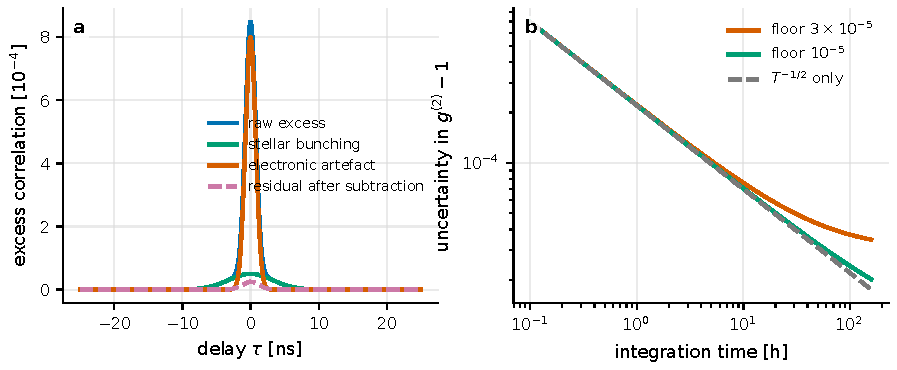
\includegraphics[width=0.96\linewidth]{figures/generated/chapter_21/ch21_calibration_artifacts.pdf}
\caption{校准误差怎样伪装成相关信号。左图中电子串扰峰比 \(5\times10^{-5}\) 的天体聚束峰大一个数量级以上，若模板扣除后还留下窄残差，就会污染 \(\hat g^{(2)}(0)\)。右图显示积分时间只按 \(T^{-1/2}\) 压低统计误差；一旦存在 \(10^{-5}\)--\(3\times10^{-5}\) 的系统误差地板，继续积分不能自动改善结论。}
\label{fig:ch21-calibration}
\end{figure}

Null test 要覆盖时间、空间、通道和积分行为。time-shift 把一路事件整体平移远大于仪器响应和天体相关宽度的时间，天体峰应消失，而慢漂移和背景结构应保留。off-source 或 off-band 换到无星光位置或不含目标谱线的频段，零延迟峰不应保留。通道置换把不应相关的探测器、偏振或光谱通道交叉相关，若仍有峰，优先怀疑串扰。分块收敛把数据按时间分成多段，相关幅度的均值应稳定，误差应按近似 \(T^{-1/2}\) 下降，直到系统地板出现。Guerin 的实验报告中，TDC 伪相关若不扣除会让 SNR 饱和；AQuEye/IquEye 文献也明确列出 SPAD 死时间、光纤延迟和环境控制对系统误差的影响 \citep{2017MNRAS.472.4126G,2016SPIE.9907E..0NZ,1996ApOpt..35.1956C,2013NIMPA.725..187J,2020RScI...91a3108W}。

\section{没有相位为什么不等于不能成像}

另一个误区是“强度干涉没有相位，所以只能测直径，不能成像”。复可见度的 Fourier 定义见第 \ref{chap:05} 章式 \eqref{eq:ch05-vcz}；强度干涉直接测的是 \(|V(u,v)|^2\)，确实丢掉了一阶复可见度相位。但 \(|V|^2\) 仍含有大量结构信息。均匀圆盘、边缘昏暗、双星、旋转扁星和简单盘面都可以直接用 \(|V|^2\) 拟合。主要困难来自退化和镜像。镜像亮度 \(I(-\boldsymbol\theta)\) 的可见度是 \(V^\ast(\boldsymbol u)\)，因此 \(|V|^2\) 完全相同；第 \ref{chap:05} 章图 \ref{fig:ch05-phase-ambiguity} 已经画出这个相位缺失问题。要分开镜像、非对称结构和复杂形态，需要多基线覆盖、物理先验、正则化 phase retrieval，或三阶相关等高阶信息 \citep{2003RPPh...66..789M,2009A&A...507.1719F,2012NewAR..56..143D,2014MNRAS.437..798M,2022MNRAS.512.1722K}。

\begin{figure}[tbp]
\centering
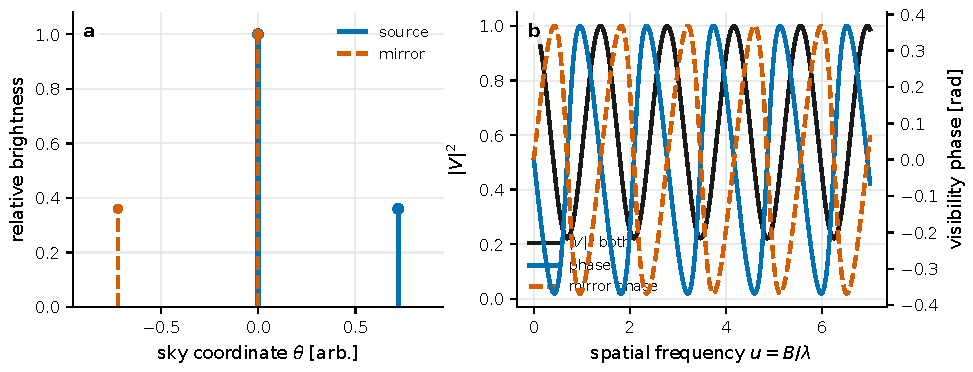
\includegraphics[width=0.96\linewidth]{figures/generated/chapter_21/ch21_phase_loss.pdf}
\caption{只测 \(|V|^2\) 的镜像退化。左图是一个不等亮双源和它的镜像；右图显示二者的 \(|V|^2\) 完全相同，但可见度相位符号相反。强度干涉可以约束结构，但需要多基线、模型先验或高阶相关来补回丢失的方向信息。}
\label{fig:ch21-phase-loss}
\end{figure}

三阶强度相关可在理想情况下给出类似闭合相位的信息，但信号比二阶相关更弱。若二阶相关的统计误差已经接近系统地板，三阶相关也会被同一批光子率和校准问题限制。大型阵列和极亮目标可以探索这个方向；第一代科学案例通常更适合从 \(|V|^2\) 的少参数模型开始，再逐步加入先验成像。

\section{量子超分辨为什么不能任意突破衍射}

SPADE 和相关模式测量纠正的是一个统计误解：Rayleigh 判据不是所有参数估计问题的信息极限。对两个弱、等亮、非相干点源，直接成像在 \(s/\sigma\ll1\) 时分离 Fisher 信息下降，而理想模式排序能保持有限 Fisher 信息 \citep{2015Optic...2..646T,2016PhRvX...6c1033T,2016OExpr..24.3684N,2017PhRvL.118g0801T}。但这不等于可以用有限光子数重建任意复杂图像。Cramér--Rao bound 和高斯 PSF 的量子 Fisher 信息已经在第 \ref{chap:08} 章式 \eqref{eq:ch08-crb} 和 \eqref{eq:ch08-qfi-gaussian} 中给出。在这些式子里，\(s\) 是要估计的角分离，单位 rad、mas 或以 PSF 宽度 \(\sigma\) 归一化；\(N_\gamma\) 是检测到并进入正确模式分析的光子数；\(F_s\) 是每个光子的 Fisher 信息，单位是角度的 \(-2\) 次方。模式测量提高的是 \(F_s\)，不能替代 \(N_\gamma\)，也不能消除背景、像差、模式串扰和质心误差。

\begin{figure}[tbp]
\centering
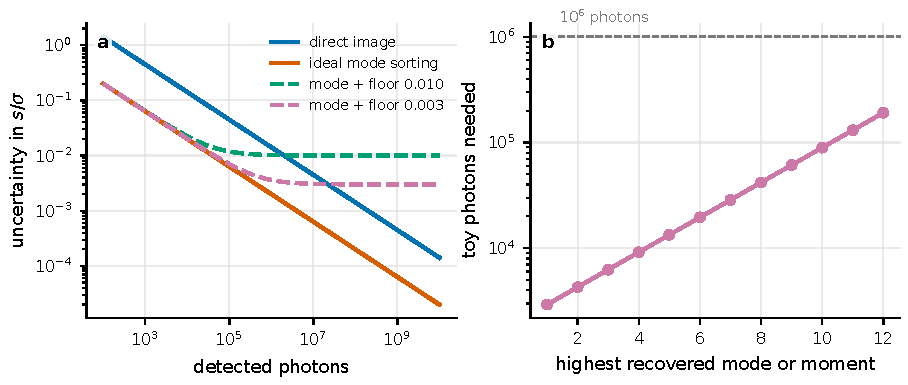
\includegraphics[width=0.96\linewidth]{figures/generated/chapter_21/ch21_superresolution_budget.pdf}
\caption{量子超分辨的光子预算和系统误差地板。左图显示 \(s=0.2\sigma\) 时直接成像和理想模式排序的统计误差标度；模式排序显著降低误差，但 \(0.003\sigma\)--\(0.01\sigma\) 的模式/质心误差地板会终止继续改善。右图用 toy model 表示恢复更高阶矩或模式所需光子数快速上升，复杂图像不能从少数光子中任意恢复。}
\label{fig:ch21-superresolution}
\end{figure}

天文语境里还要区分源本身的相干性和传播后的一阶空间相干。部分相干源会改变模式概率，相关文献中对 Rayleigh curse 是否重新出现的讨论围绕这个条件展开 \citep{2017NJPh...19b3054T,2017PhRvA..95f3847A,2018Optic...5.1177P,2018Optic...5.1382L,2019Optic...6..400T}。因此，把“两点非相干高斯源”的结论直接推广到星系、吸积盘、喷流或强透镜弧会失去适用条件。给定源模型、PSF、背景和测量基后，模式测量可以提高某些参数的信息效率；离开这些条件，超分辨只是一个口号。

\section{天体 laser、maser 和非 Poisson 统计最容易混淆在哪里}

“天体 laser/maser 一定有 \(g^{(2)}=1\)”也是误区。受激辐射可以产生高亮温、窄线和强偏振，但天体环境通常没有实验室稳定谐振腔。未饱和 maser、饱和 maser、速度相干路径、泵浦涨落、多个斑点叠加和连续谱背景都会改写光子统计 \citep{1982RvMP...54.1225E,1992ARA&A..30...75E,1985ARA&A..23..169D}。Eta Carinae 的 Weigelt blobs 中，Fe II 和 O I 线的自然激光候选需要同时看 Ly\(\alpha\) 泵浦、能级反转、线宽、空间位置和连续谱扣除；Brown--Twiss--Townes heterodyne correlation 被提出用来测窄 Fe II 线宽 \citep{2004A&A...428..497J,2005MNRAS.364..731J,2005NewA...10..361J,2008AIPC..984..216D}。

若观测光由多个独立成分叠加，总强度 \(I=\sum_a I_a\)，且不同成分之间没有强度相关，则零延迟相关超额近似为
\begin{equation}
  g_{\rm mix}^{(2)}(0)-1
  =
  \sum_a f_a^2\left[g_a^{(2)}(0)-1\right],
  \qquad
  f_a=\frac{\langle I_a\rangle}{\sum_b\langle I_b\rangle}.
  \label{eq:ch21-mixture}
\end{equation}
\begin{formulaexplain}[公式 (21.2) 解读]
\(f_a\) 是第 \(a\) 个成分的通量分数。相关超额按 \(f_a^2\) 加权，所以少量热连续谱或多成分混合会把 \(g^{(2)}\) 解释变得很危险。
\end{formulaexplain}
\(f_a\) 是通量分数，无量纲。一个占总通量 \(20\%\) 的热成分，即使自身 \(g^{(2)}(0)-1=1\)，混合后也只贡献 \(0.04\) 的对比度；若再有 \(M=100\) 个模式和 \(\tau_c/\Delta t=10^{-5}\)，观测对比度变成 \(4\times10^{-9}\)。反过来，未饱和受激线若带有泵浦强度噪声，可能产生超 Poisson 统计；这种结果要先分离谱线、连续谱和仪器响应，不应直接归因于新物理。

\begin{figure}[tbp]
\centering
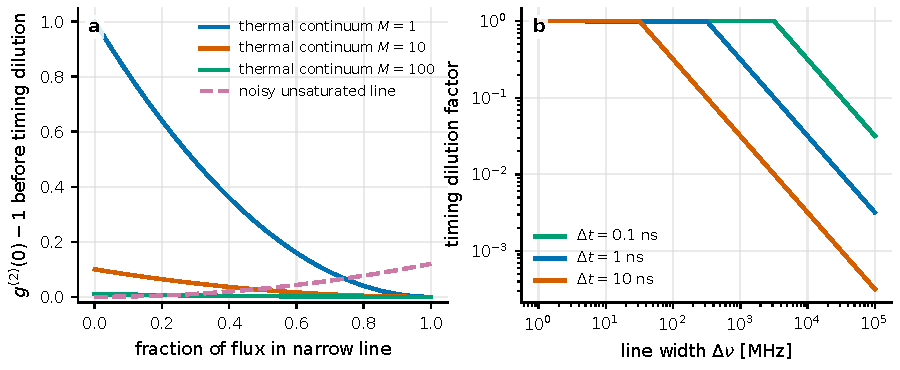
\includegraphics[width=0.96\linewidth]{figures/generated/chapter_21/ch21_maser_mixed_statistics.pdf}
\caption{天体 maser/laser 候选中的混合统计。左图显示窄线通量分数增加时，热连续谱聚束按通量分数平方被稀释；若窄线本身有未饱和强度噪声，则会出现另一条超 Poisson 分支。右图显示谱线宽度和电子学时间 bin 对相关对比度的稀释，MHz--GHz 线宽需要 ns 或更快的时间响应才能保留较大峰值。}
\label{fig:ch21-maser}
\end{figure}

非 Poisson 统计同样有普通来源。一个随机变源可以看成 Cox process：在给定瞬时率 \(\Lambda\) 时计数是 Poisson，但 \(\Lambda\) 本身随时间或环境变化。于是
\begin{equation}
  F_{\rm Fano}
  \equiv \frac{{\rm Var}(N)}{\mathbb E(N)}
  =
  1+\frac{{\rm Var}(\Lambda)}{\mathbb E(\Lambda)}
  \label{eq:ch21-fano}
\end{equation}
\begin{formulaexplain}[公式 (21.3) 解读]
\(F_{\rm Fano}\) 是方差与均值之比。若瞬时率 \(\Lambda\) 自身在变，计数会自然变成 super-Poisson，不必先诉诸非经典光源。
\end{formulaexplain}
在合适时间 bin 中大于 1。死时间会压低短间隔事件，使 \(F_{\rm Fano}<1\) 或在短延迟出现负相关；afterpulsing 会在探测器特征时间后产生正相关。第六章给出的 afterpulsing 概率 \(10^{-4}\)--\(10^{-2}\) 已足以污染许多短延迟搜索。判断“非 Poisson”之前，应先画 Fano factor 随 bin 宽变化、短延迟自相关和互相关、暗场数据、off-source 数据以及 time-shift 背景。

\begin{figure}[tbp]
\centering
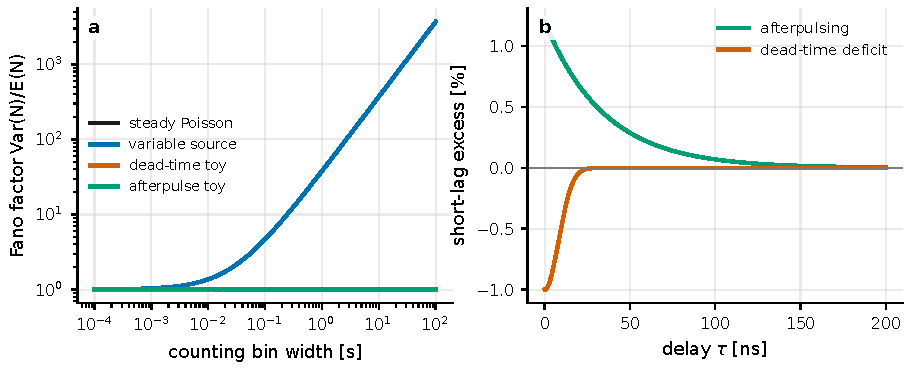
\includegraphics[width=0.96\linewidth]{figures/generated/chapter_21/ch21_nonpoisson_diagnostics.pdf}
\caption{非 Poisson 统计的普通来源。左图用 Fano factor 展示稳态 Poisson、慢变源、死时间和 afterpulsing 的不同标度；慢变源在长 bin 中变得 super-Poisson，死时间造成 under-dispersion。右图显示 afterpulsing 和死时间在短延迟相关函数中的相反形状，这些仪器特征应先从暗场和交叉通道中量化。}
\label{fig:ch21-nonpoisson}
\end{figure}

\section{假警报怎样画出新物理边界}

单次小概率事件也常被误读为发现。若一次检验的尾概率是 \(p_0\)，独立试验数为 \(N_{\rm trial}\)，至少出现一次的概率是
\begin{equation}
  p_{\rm any}=1-(1-p_0)^{N_{\rm trial}}
  \simeq N_{\rm trial}p_0
  \quad (N_{\rm trial}p_0\ll1).
  \label{eq:ch21-trials}
\end{equation}
\begin{formulaexplain}[公式 (21.4) 解读]
\(p_0\) 是单次检验的尾概率，\(N_{\rm trial}\) 是试验次数。搜索空间越大，至少看到一次偶然峰的概率越高，因此要报告全局显著性。
\end{formulaexplain}
\(N_{\rm trial}\) 可以来自时间 bin 数、频率通道数、基线数、目标数、模型网格和事后挑选的窗口。若每晚搜索 \(10^6\) 个候选延迟/频率/目标组合，单次 \(p_0=10^{-5}\) 的事件几乎必然会出现。多重检验不是形式主义；它决定一个峰是天文信号、仪器异常还是搜索空间中的自然尾部。

\begin{figure}[tbp]
\centering
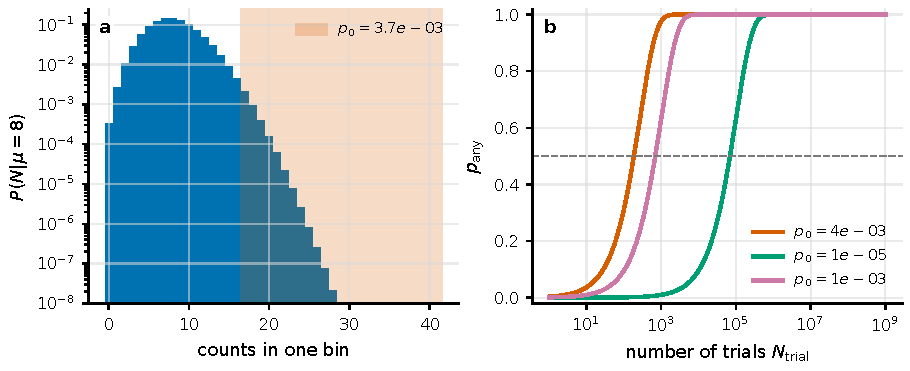
\includegraphics[width=0.96\linewidth]{figures/generated/chapter_21/ch21_poisson_false_alarm.pdf}
\caption{Poisson 尾部和多重检验。左图中 \(\mu=8\) 的单个 bin 偶尔会出现 \(N\ge17\) 的高计数尾部；右图显示同样的单次 \(p_0\) 在大量 trial 中如何变成很高的全局假警报概率。事件表搜索、周期搜索、跨频相关和暂现源筛选都要报告 \(N_{\rm trial}\) 或等效全局显著性。}
\label{fig:ch21-false-alarm}
\end{figure}

“量子天文学”也不等于“量子引力”。前面大部分内容研究的是光场统计、模式测量、相干函数、仪器和信息极限。黑洞、CMB、轴子、宇宙双折射或暗物质透镜可以进入这条主线，是因为它们能写成可观测的时间、频率、偏振或空间相关量，并非因为每个话题都需要 Planck 尺度物理。一个可检查的异常信号需要把数据来源拆开：
\begin{equation}
  d_{\rm obs}=d_{\rm sky}(\boldsymbol\theta)
  +d_{\rm inst}(\boldsymbol\phi)
  +d_{\rm sel}(\boldsymbol\psi)
  +n,
  \label{eq:ch21-data-model}
\end{equation}
\begin{formulaexplain}[公式 (21.5) 解读]
\(d_{\rm obs}\) 是观测数据，右边把天空、仪器、选择函数和噪声分开。任何“新物理”解释都应先证明普通天体项和仪器项不能解释数据。
\end{formulaexplain}
其中 \(d_{\rm obs}\) 是数据向量，例如延迟直方图、\(|V|^2\)、偏振相关或事件时间；\(d_{\rm sky}\) 是天体模型；\(d_{\rm inst}\) 是仪器模型；\(d_{\rm sel}\) 是选择函数；\(n\) 是噪声。若这四项还没有分开，异常峰、偏振旋转或非 Poisson 计数都不应直接归因于新物理。

研究计划的最后一页应回到新增观测量：它是平均强度、二阶相关、跨频协方差、偏振相关，还是模式计数。若目标是二阶相关，就列出事件表怎样生成延迟直方图、time-shift 背景怎样定义、零延迟峰怎样标定；若目标是偏振或模式计数，就列出通道定义、响应矩阵、背景项和协方差。每个量都要配上单位、典型范围和适用条件，例如热光、高斯 PSF、弱光、少参数源模型或稳定仪器响应。null test 至少应从 time-shift、off-source、off-band、暗场、错偏振和注入恢复中选出两个；全局显著性和系统误差地板要同时进入结论。

